\documentclass[uplatex]{jsarticle}

% パッケージ
\usepackage[dvipdfmx]{hyperref, graphicx}
\usepackage{pxjahyper}
\usepackage{siunitx} % SI単位
\usepackage{amssymb}
\usepackage{amsmath}
\usepackage{caption,subcaption}
\usepackage[top=20truemm,bottom=20truemm,left=25truemm,right=25truemm]{geometry}
\usepackage{here}
\usepackage{ascmac} % 枠付き文章


\hypersetup{
    colorlinks=false, % リンクに色をつけない設定
    bookmarks=true, % 以下ブックマークに関する設定
    bookmarksnumbered=true,
    pdfborder={0 0 0},
    bookmarkstype=toc,
}

\newcommand{\linedhref}[2]{\underline{\href{#1}{\emph{#2}}}}

% 接頭辞の設定
\renewcommand{\figurename}{Fig.}
\renewcommand{\tablename}{Table.}
\newcommand\figref[1]{{図~\ref{fig:#1}}}
\newcommand\tabref[1]{{表~\ref{tab:#1}}}
\newcommand\eref[1]{{式~({\boldmath \ref{eq:#1}})}}
\newcommand\secref[1]{{第~\ref{sec:#1}章}}
\newcommand\ssecref[1]{{~\ref{sec:#1}節}}
\def\abstractname{要旨}
\def\prepartname{第}
\def\postpartname{章}

% 自作関数
\newcommand{\divergence}{\mathrm{div}\,}  %ダイバージェンス
\newcommand{\grad}{\mathrm{grad}\,}  %グラディエント
\newcommand{\rot}{\mathrm{rot}\,}  %ローテーション
\def\vector#1{\mbox{\boldmath $#1$}}
\newcommand{\e}{\mathrm{e}} %自然対数
\newcommand{\pdiff}[3]{
    \if 1#1 \dfrac{\partial #2}{\partial #3}
    \else \dfrac{\partial^{#1} #2}{\partial #3^{#1}}\fi
}

% Captionの設定
% \captionwidth=0.8\textwidth
\captionsetup[figure]{font=small}
\captionsetup[table]{font=small} %small=9pt,footnotesize=8pt}
\abovecaptionskip=5pt
\belowcaptionskip=0pt
\title{\LaTeX のサンプルソース}
\author{a11-green}

\begin{document}
\maketitle
\tableofcontents

\newpage
\section{はじめに}
この文書は本テンプレートで作成する\LaTeX 文書のサンプルと、ここで使える文法の確認を兼ねたものである。
各種コマンドを使用するために必要なパッケージを指定するプリアンブル部および自作関数(コマンド)の定義部、各種文書設定などの共通部分はsetting.texに別ファイルとしてまとめ、ドキュメント本文の冒頭でinput文によって挿入することで視認性および管理のしやすさを上げることができる。
本Docker環境にはTexLiveを用いているため、TexLiveにはじめから同梱されているパッケージについてはusepackageによる宣言のみで使用することができる。
上記に当てはまらないパッケージについては各自Dockerfile内にtlmgrによるインストールコマンドを記述する必要がある。tlmgrによるインストールを行う際には最新のTexLiveを使用することが簡単であり望ましい。

\section{基本文法}
\subsection{文と数式}
文章は日本語で書くことができる\footnote{注釈をフッターに記述することもできる。}。
また文章を枠で囲む場合はitembox文などを利用することができる\cite{itembox}:
\begin{itembox}[l]{Fermatの最終定理}
3以上の自然数$n$について$x^n+y^n=z^n$となる自然数の組$(x,y,z)$は存在しない。
\end{itembox}
単位についてはsi文を用いることでrm文による立体化などの手間を省くことができる。
たとえば体積流量の単位は 99 \si{m^3/min}のように記述する。単位の前にはスペースを空けることを推奨する。
\par
数式は\eref{mass-conservation}のようにalign環境やequation環境などを用いて記述する:
\begin{align}
	\pdiff{1}{u}{x} + \pdiff{1}{v}{y} + \pdiff{1}{w}{z} = 0
	\label{eq:mass-conservation}
\end{align}
式の参照について、式にラベルをつける際に接頭辞としてeq:をつけておくことで視認性を上げるとともに、自作関数であるeref文によりeq:の後の文字列を指定することで式(・)として参照できるようにしている。
またよく使う偏微分は自作関数のpdiff文で簡単に記述できるようにしている。
詳しくはsetting.texを参照されたい。



\subsection{図}
図を挿入するためのコマンドを全部手で打つのは面倒なので、頻繁に使うものに関しては.vscode/latex.code-snippets中にユーザスニペットとして登録しており、fig1と入力することでvscodeによって候補が提示されるのでそれを選択することでテンプレートを挿入することができる。例えば1枚の図を挿入する場合は次のようになる:
\begin{figure}[H]
	\centering
	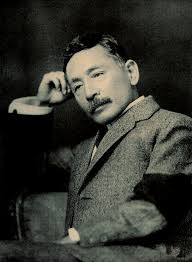
\includegraphics[width=0.2\textwidth]{figure/natsume_soseki.jpeg}
	\caption{夏目漱石の写真\cite{Soseki1905}。1枚の場合。}
	\label{fig:夏目漱石の写真}
\end{figure}
同様に2舞の場合は次のようになる:
\begin{figure}[H]
	\centering
	\begin{minipage}[b]{0.49\linewidth}
		\centering
		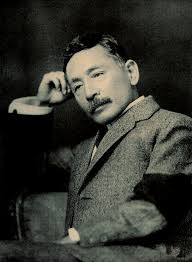
\includegraphics[width=0.6\textwidth]{figure/natsume_soseki.jpeg}
		\subcaption{1枚目}
		\label{fig:first}
	\end{minipage}
	\begin{minipage}[b]{0.49\linewidth}
		\centering
		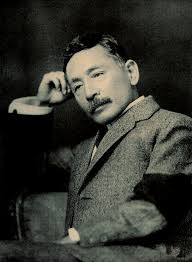
\includegraphics[width=0.6\textwidth]{figure/natsume_soseki.jpeg}
		\subcaption{2枚目}
		\label{fig:second}
	\end{minipage}
	\caption{夏目漱石の写真\cite{Soseki1905}。2枚の場合。}
	\label{fig:}
\end{figure}

\par
label文によって図にラベルを付ける場合はfig:を接頭辞として指定する。
このとき図の参照はfig:の後の文字列を自作関数のfigref文で指定することで図(・)として参照できる(例えば\figref{second})。

\subsection{表}



\bibliography{ref}
\bibliographystyle{junsrt}
% \bibliographystyle{ieeepes}
参考文献はbibtexによって記述する。
本文中では参照するbibファイルと表示するスタイルを指定する。
記述内容は例えばarXivなどであれば用意されているためそれをそのまま転記すればよい。
mendeleyやpaperpileなどからまとめて自動作成するようにしておけばさらに便利である。
スタイルについては論文誌などで指定があればそれに従い、特に指定がなければお気に入りのものを探すとよい。

\end{document}